\documentclass[11pt]{beamer}
\usetheme{Warsaw}
\usepackage[utf8]{inputenc}
\usepackage[vietnamese]{babel}
\usepackage{amsmath}
\usepackage{amsfonts}
\usepackage{amssymb}
\usepackage{graphicx}
\usepackage{caption}
\usepackage{booktabs}

%
\author{Nguyễn Hoàng Đức, Lê Nhựt Nam, Nguyễn Viết Dũng}
\title{VOICE BIOMETRICS}
\institute{Đại học Khoa học Tự nhiên, Đại học Quốc Gia TP HCM} 

%
\setbeamertemplate{caption}[numbered]
\setbeamertemplate{footline}[frame number]

%
\newcommand{\argmax}{\arg\!\max}

\begin{document}

\begin{frame}
\titlepage
\end{frame}
\begin{frame}{Nội dung trình bày}
	\textbf{A. Trình bày nội dung tìm hiểu được từ Chapter 8 - Voice Biometrics}
	\begin{itemize}
		\item Giới thiệu
		\item Xác định những thông tin trong tín hiệu giọng nói
		\item Rút trích đặc trưng và Phân tách dữ liệu
		\item Nhận dạng giọng nói phụ thuộc văn bản
		\item Nhận dạng giọng nói không phụ thuộc văn bản
		\item Ứng dụng
	\end{itemize}
\end{frame}
\begin{frame}{Nội dung trình bày}
	\textbf{B. Trình bày các phương pháp STATE OF THE ART của Voice Recognition}
	\begin{itemize}
		\item Mục đích
		\item Động lực nghiên cứu khoa học 
		\item Phát biểu bài toán
		\item Các công trình liên quan
		\item Phương pháp giải thuật
		\item Demo
		\item Tài liệu tham khảo
	\end{itemize}
\end{frame}

\section{Chapter 8 - Voice Biometrics}
\subsection{Giới thiệu về Sinh trắc học Giọng nói}
\begin{frame}{Giới thiệu}
	\begin{itemize}
		\item Giọng nói (Voice/Speech) là một đặc điểm sinh trắc học (nhân trắc học) dễ dàng tiếp cận nhất mà không cần phải có thêm thiết bị thu nhận và hệ thống truyền dẫn.
		\item Có lợi thế khi áp dụng vào các hệ thống điều khiển từ xa
		\item Giọng nói không chỉ liên quan đến các đặc trưng cá thể mà còn liên quan với môi trường xung quanh và vấn đề xã hội, do vậy việc sản sinh giọng nói là một kết quả của một quá trình hết sức phức tạp.
	\end{itemize}
\end{frame}
\subsection{Xác định những thông tin trong tín hiệu giọng nói}
\begin{frame}{Idiolectal characteristics}
	Idiolectal = idio (personal, private) + (dia)lect
	\begin{itemize}
		\item Thói quen nói đặc biệt của một người cụ thể.
		\item Một "Idiolectal" là lời nói đặc biệt của một cá nhân, một ngôn ngữ được coi là duy nhất trong số những người nói ngôn ngữ hoặc phương ngữ của một người. Nhưng nó thậm chí còn hẹp hơn nhiều so với tất cả những người nói một phương ngữ cụ thể.
		\item Ngôn ngữ đa dạng duy nhất cho một người nói một ngôn ngữ được gọi là idiolect. idiolect của bạn bao gồm các từ vựng phù hợp với các sở thích và hoạt động khác nhau của bạn, cách phát âm phản ánh khu vực bạn đang sống hoặc đã sống và các phong cách nói khác nhau thay đổi một cách tinh vi tùy thuộc vào người bạn đang nói đến
	\end{itemize}
\end{frame}
\begin{frame}{Phonotactics characteristics}
	\begin{itemize}
		\item Ngữ âm là một phần của âm vị học của một ngôn ngữ.
		\item Ngữ âm hạn chế các chuỗi âm thanh và cấu trúc âm tiết có thể có trong một ngôn ngữ.
		\item Ràng buộc phonotactic đề cập đến bất kỳ hạn chế cụ thể nào.
	\end{itemize}
\end{frame}
\begin{frame}{Prosody characteristics}
	\begin{itemize}
		\item Trong ngôn ngữ học, prosody quan tâm đến những yếu tố của lời nói không phải là các phân đoạn ngữ âm riêng lẻ (nguyên âm và phụ âm) mà là thuộc tính của âm tiết và các đơn vị lớn hơn của lời nói, bao gồm các chức năng ngôn ngữ như như ngữ điệu, giai điệu, trọng âm và nhịp điệu. Các phần tử như vậy được gọi là siêu phân đoạn.
		\item Introduction 2
		\item Introduction 3
	\end{itemize}
\end{frame}
\begin{frame}{Short-term spectral characteristics}
	\begin{itemize}
		\item Introduction 1
		\item Introduction 2
		\item Introduction 3
	\end{itemize}
\end{frame}

\subsection{Rút trích đặc trưng và phân tách dữ liệu}
\begin{frame}{Introduction}
	\begin{itemize}
		\item Introduction 1
		\item Introduction 2
		\item Introduction 3
	\end{itemize}
\end{frame}
\subsubsection{Phân tích trong thời gian ngắn}
\begin{frame}{Introduction}
	\begin{itemize}
		\item Introduction 1
		\item Introduction 2
		\item Introduction 3
	\end{itemize}
\end{frame}
\begin{frame}{Introduction}
	\begin{figure}[h!]
		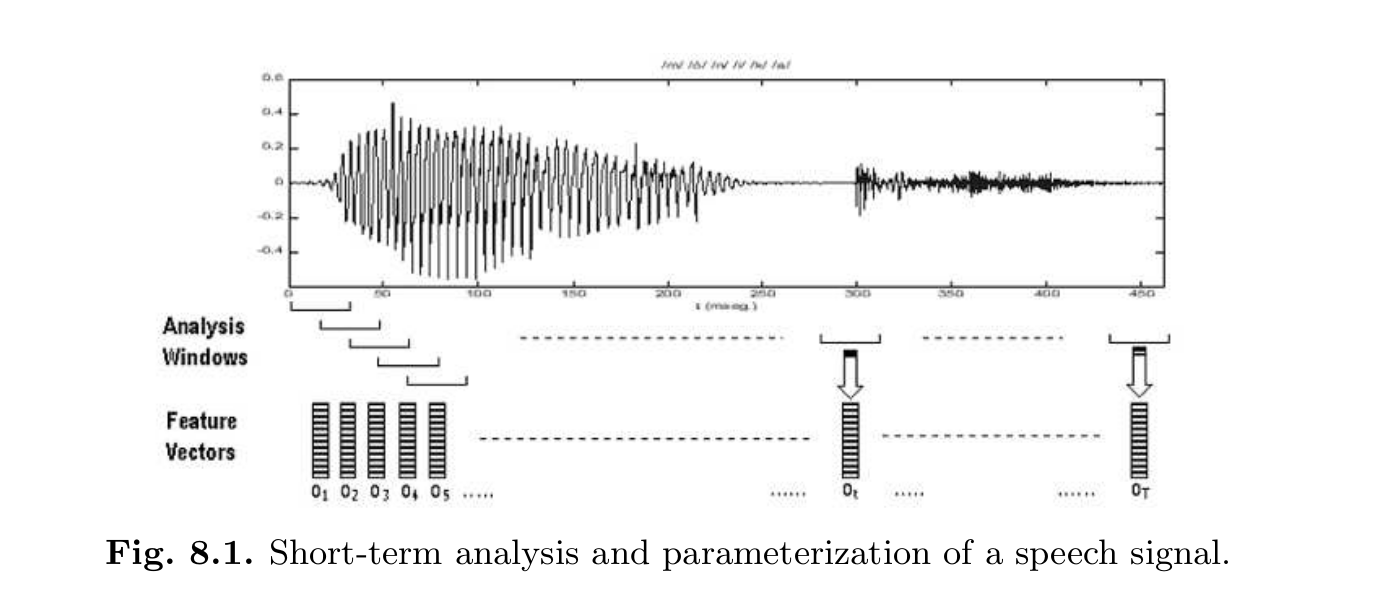
\includegraphics[width=0.9\linewidth]{images/figure_8_1.png}
		\caption{Handbook of Biometrics, page 155}
		\label{fig:writing-thesis}
	\end{figure}
\end{frame}

\subsubsection{Tham số hóa}
\begin{frame}{Introduction}
	\begin{itemize}
		\item Introduction 1
		\item Introduction 2
		\item Introduction 3
	\end{itemize}
\end{frame}
\subsubsection{Phân tích ngữ âm và tách từ}
\begin{frame}{Introduction}
	\begin{itemize}
		\item Introduction 1
		\item Introduction 2
		\item Introduction 3
	\end{itemize}
\end{frame}
\subsubsection{Phân tách ngữ điệu}
\begin{frame}{Introduction}
	\begin{itemize}
		\item Introduction 1
		\item Introduction 2
		\item Introduction 3
	\end{itemize}
\end{frame}

\subsection{Nhận dạng giọng nói phụ thuộc văn bản}
\begin{frame}{Related works}
\end{frame}

\subsection{Nhận dạng giọng nói không phụ thuộc văn bản}
\begin{frame}{Related works}
\end{frame}
\subsubsection{Hệ thống phổ trong thời gian ngắn}
\begin{frame}{Introduction}
	\begin{itemize}
		\item Introduction 1
		\item Introduction 2
		\item Introduction 3
	\end{itemize}
\end{frame}
\subsubsection{Hệ thống Idiolectal}
\begin{frame}{Introduction}
	\begin{itemize}
		\item Introduction 1
		\item Introduction 2
		\item Introduction 3
	\end{itemize}
\end{frame}
\subsubsection{Hệ thống ngữ âm}
\begin{frame}{Mô hình hệ thống ngữ âm}
	\begin{figure}[h!]
		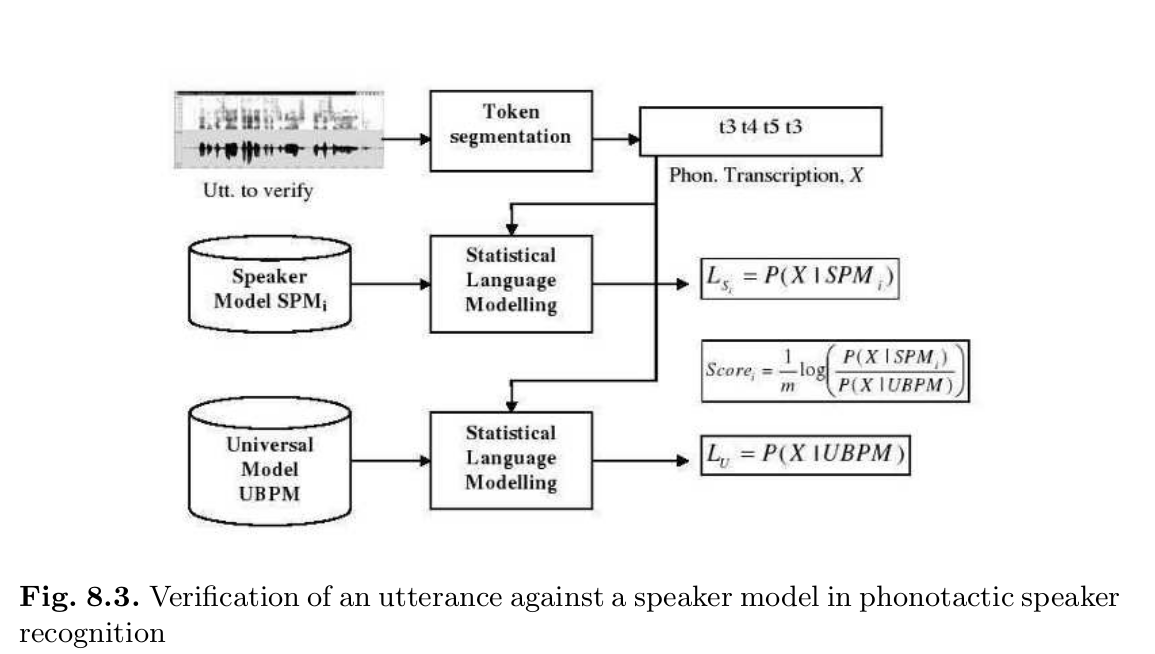
\includegraphics[width=0.9\linewidth]{images/figure_8_3.png}
		\caption{Handbook of Biometrics, page 162}
		\label{fig:writing-thesis}
	\end{figure}
\end{frame}	
\subsubsection{Hệ thống ngữ điệu}
\begin{frame}{Mô hình hệ thống ngữ điệu}
	\begin{figure}[h!]
		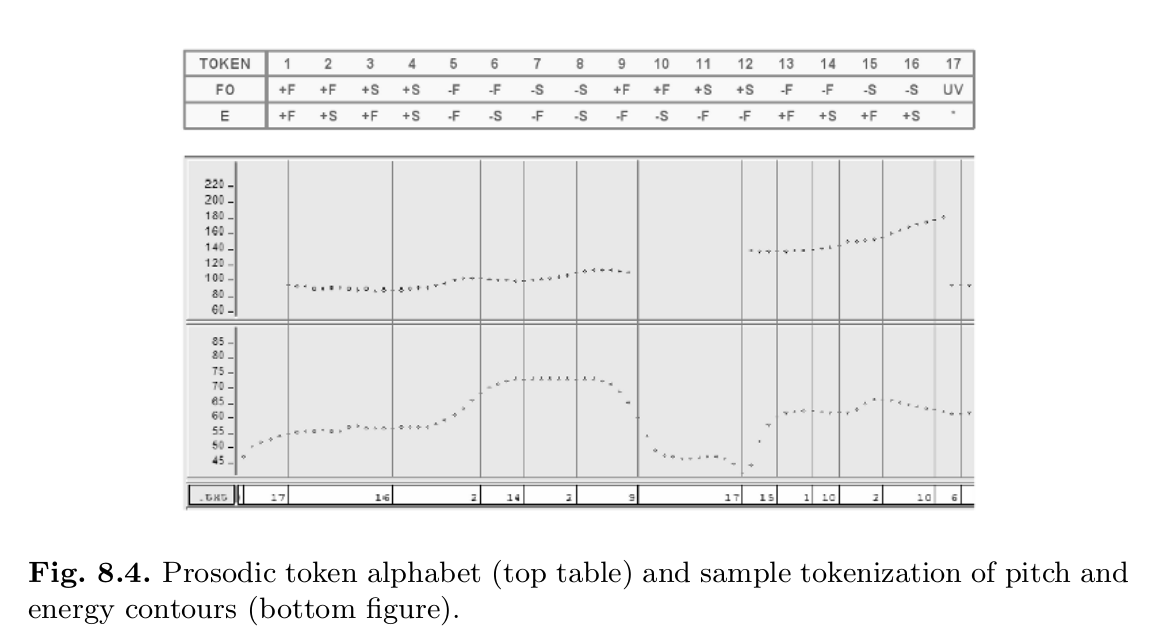
\includegraphics[width=0.9\linewidth]{images/figure_8_4.png}
		\caption{Handbook of Biometrics, page 163}
		\label{fig:writing-thesis}
	\end{figure}
\end{frame}	
\subsection{Ứng dụng}
\begin{frame}{Voice authentication}
	\begin{figure}[h!]
		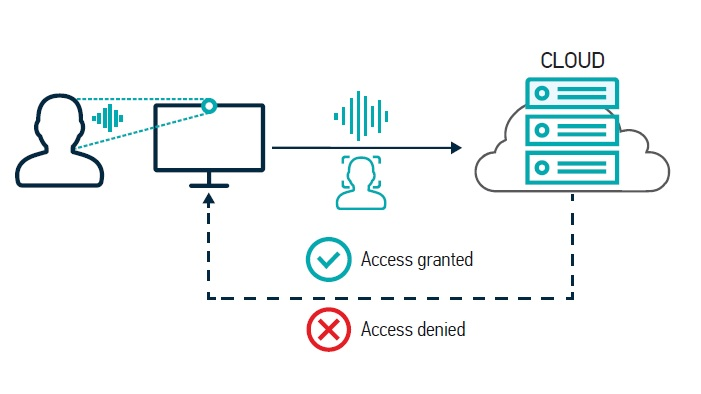
\includegraphics[width=0.9\linewidth]{images/voice_authentication.jpg}
		\caption{Ví dụ Voice authentication/ Verification}
		\label{fig:writing-thesis}
	\end{figure}
\end{frame}	
\begin{frame}{Speaker Identification and Verification}
	\begin{figure}[h!]
		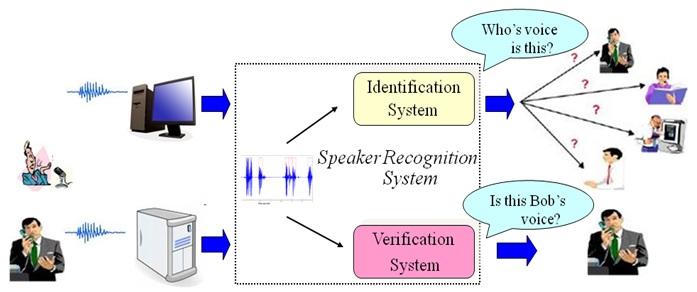
\includegraphics[width=0.9\linewidth]{images/speaker_identification_verification.jpeg}
		\caption{Ví dụ Speaker Recognition Systems}
		\label{fig:writing-thesis}
	\end{figure}
\end{frame}
\begin{frame}{Forensic speaker recognition}
	\begin{figure}[h!]
		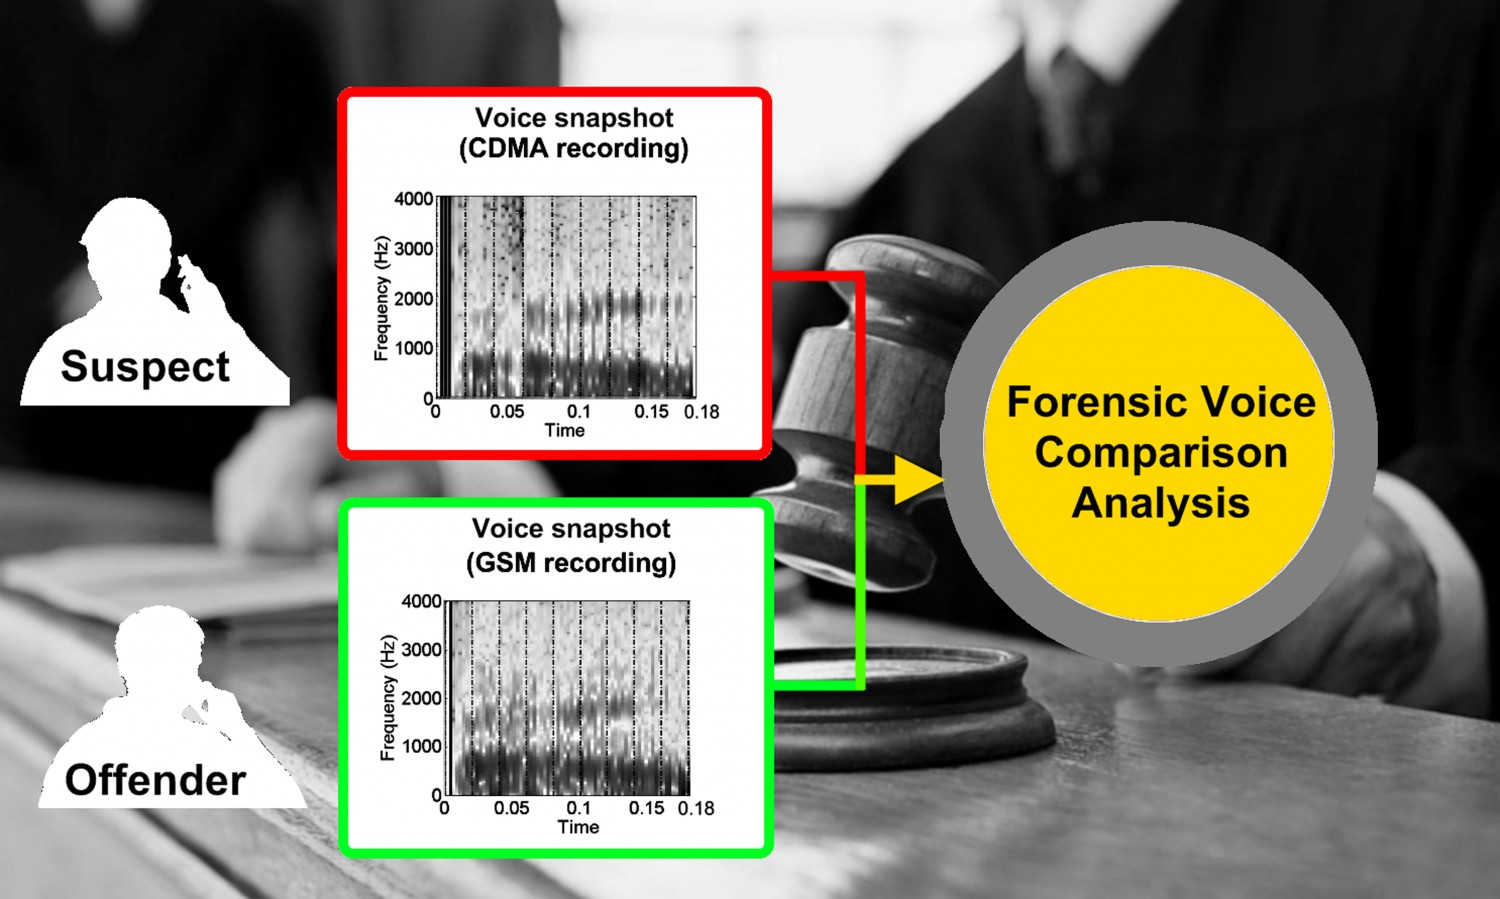
\includegraphics[width=0.9\linewidth]{images/forensic_voice.jpg}
		\caption{Ví dụ Speaker Recognition Systems}
		\label{fig:writing-thesis}
\end{figure}
\end{frame}

\section{Các phương pháp Voice Biometrics}
\subsection{Động lực nghiên cứu khoa học - Motivation}
\begin{frame}{Related works}
\end{frame}
\subsection{Phát biểu bài toán - Problem statment}
\begin{frame}{Phát biểu bài toán}
	\textbf{Tác vụ:} Định danh người nói
	\begin{itemize}
		\item Đầu vào (Input): Dữ liệu âm thanh giọng nói
		\item Đầu ra (Output): Danh tính của người nói
	\end{itemize}
	\textbf{Tác vụ:} Xác nhận người nói
	\begin{itemize}
		\item Đầu vào (Input): Dữ liệu âm thanh giọng nói
		\item Đầu ra (Output): Đồng ý/ Từ chối
	\end{itemize}
\end{frame}
\subsection{Các công trình liên quan - Related Work}
\begin{frame}{Related works}
	
\end{frame}
\subsection{Phương pháp giải thuật - Methods}
\begin{frame}{Related works}
\end{frame}
\subsection{Demo}
\begin{frame}{Related works}
\end{frame}
\subsection{Tài liệu tham khảo - References}
\begin{frame}
	\nocite{*}
	\bibliography{references}\newpage\cleardoublepage
	\bibliographystyle{plain}
\end{frame}

\end{document}